%
%                       This is a basic LaTeX Template
%                       for the Informatics Research Review

\documentclass[a4paper,11pt]{article}
% Add local fullpage and head macros
\usepackage{head,fullpage}     
% Add graphicx package with pdf flag (must use pdflatex)
\usepackage[pdftex]{graphicx}  
% Better support for URLs
\usepackage{url}
% Date formating
\usepackage{datetime}

\usepackage{subcaption}

\usepackage[colorlinks=true, allcolors=blue]{hyperref}

\usepackage[format=plain,
            labelfont=it,
            textfont=it]{caption}


\newdateformat{monthyeardate}{%
  \monthname[\THEMONTH] \THEYEAR}

\parindent=0pt          %  Switch off indent of paragraphs 
\parskip=5pt            %  Put 5pt between each paragraph  
\Urlmuskip=0mu plus 1mu %  Better line breaks for URLs


%                       This section generates a title page
%                       Edit only the following three lines
%                       providing your exam number, 
%                       the general field of study you are considering
%                       for your review, and name of IRR tutor

\newcommand{\examnumber}{B203937}
\newcommand{\field}{CNNs in Digital Art Restoration}
\newcommand{\supervisor}{Pavlos Andreadis}

\begin{document}
\captionsetup[table]{labelfont=it,textfont={it}}
\captionsetup[figure]{labelfont=it,textfont={it}}
\begin{minipage}[b]{110mm}
        {\Huge\bf School of Informatics
        \vspace*{17mm}}
\end{minipage}
\hfill
\begin{minipage}[t]{40mm}               
        \makebox[40mm]{
        \includegraphics[width=40mm]{crest.png}}
\end{minipage}
\par\noindent
    % Centre Title, and name
\vspace*{2cm}
\begin{center}
        \Large\bf Informatics Research Review \\
        \Large\bf \field
\end{center}
\vspace*{1.5cm}
\begin{center}
        \bf \examnumber\\
        \monthyeardate\today
\end{center}
\vspace*{5mm}

%
%                       Insert your abstract HERE
%                       
\begin{abstract}
       Many forms of artwork suffer damage over time due to humidity, light exposure, vandalism, or natural aging. While efforts have been made to restore these artworks by hand, technological reproductions have become more popular recently in order to avoid damage caused by human error. One such solution is the Convolutional Neural Network (CNN). This essay aims to evaluate the ways in which CNNs have improved the quality of digital reproductions compared to previous computer-based methods. It does so by examining the CNN's performance on subtasks, as well as critically analysing the flexibility and accessibility of this deep learning tool. 
\end{abstract}

\vspace*{1cm}

\vspace*{3cm}
Date: \today

\vfill
{\bf Supervisor:} \supervisor
\newpage

%                                               Through page and setup 
%                                               fancy headings
\setcounter{page}{1}                            % Set page number to 1
\footruleheight{1pt}
\headruleheight{1pt}
\lfoot{\small School of Informatics}
\lhead{Informatics Research Review}
\rhead{- \thepage}
\cfoot{}
\rfoot{Date: \date{\today}}
%

\section{Introduction}
 
Art is an integral part of our society and history. From wall paintings of religious figures to ink sketches of architecture, art reflects trends in human culture across time, and is sometimes the only depiction of life and philosophy from which we can draw historical conclusions. However, due to poor weather conditions, light exposure, or merely the natural aging process of the materials with which the art was created, art can undergo moderate to severe degradation over time \cite{barni2005}\cite{gupta}\cite{amiri}. As such, intensive restoration is required to bring these artworks back to their former beauty.

Art restoration is traditionally performed by hand under the keen and careful skill of professional artists. And while this method has generally achieved great success, one painting may take months— or even years to be restored \cite{amiri}. Acquiring the proper resources (tools, artists, etc.) for restoration creates additional financial and accessibility burdens \cite{barni2000}. Of course, there is always the risk of a 'botched' reproduction or damage to the original too, such as with Figure 1 \cite{jesus}. For this reason, scientists and artists turned to technological reconstructions, which can not only help guide the physical restoration process while minimizing risk of damage to the original, but also provide a reproducible digital image that can be easily shown to viewers \cite{barni2005}.

In early attempts to automate the art restoration process, scientists relied on fully formed neural networks and/or statistical analysis to re-imagine artwork \cite{barni2000}\cite{palomero}\cite{giakoumis}\cite{spagnolo}. However, statistically-based methods were often limited in scope, and did not conform well to human mental models \cite{gupta}. Also, traditional neural networks were inefficient, since features had to be hard-coded \cite{sizyakin}. These logistical flaws make both of these methods incompatible with the complex, high resolution patterns that are so common in today's research \cite{sizyakin}. On the other hand, deep learning methods such Convolutional Neural Networks (CNNs) extract their own features, are cost-effective, and can manipulate artwork in smarter and more efficient ways to produce better results. They can also be entirely virtual, which gives them an advantage over other technological solutions which require physical aid.  

This literature review aims to evaluate the extent to which CNNs have improved the quality and accessibility of digitally restored art, and thus enhance our understanding of past artifacts. Since art restoration is a complex task with many steps, we will focus our review by comparing the performance of CNNs with other methods (kNN, Linear Regression) on three main restoration subtasks: color restoration, crack detection, and image inpainting. These subtasks were chosen because they are the most prevalent issues in art restoration— as such, they are also the most widely studied \cite{barni2005}. In order to illustrate the vast applications of digital restoration, the artworks sampled here include ancient cave paintings, oil paintings from the 1600-1800s, and ink drawings from the 1800s. Processing of real photographs, although used in some of the chosen literature, will not be considered in-depth here, nor will we consider other subtasks like super-resolution or image deblurring. Finally, in later sections, we save space for forward thinking, and consider the trajectory of future research.

\begin{figure}[h]
    \centering
    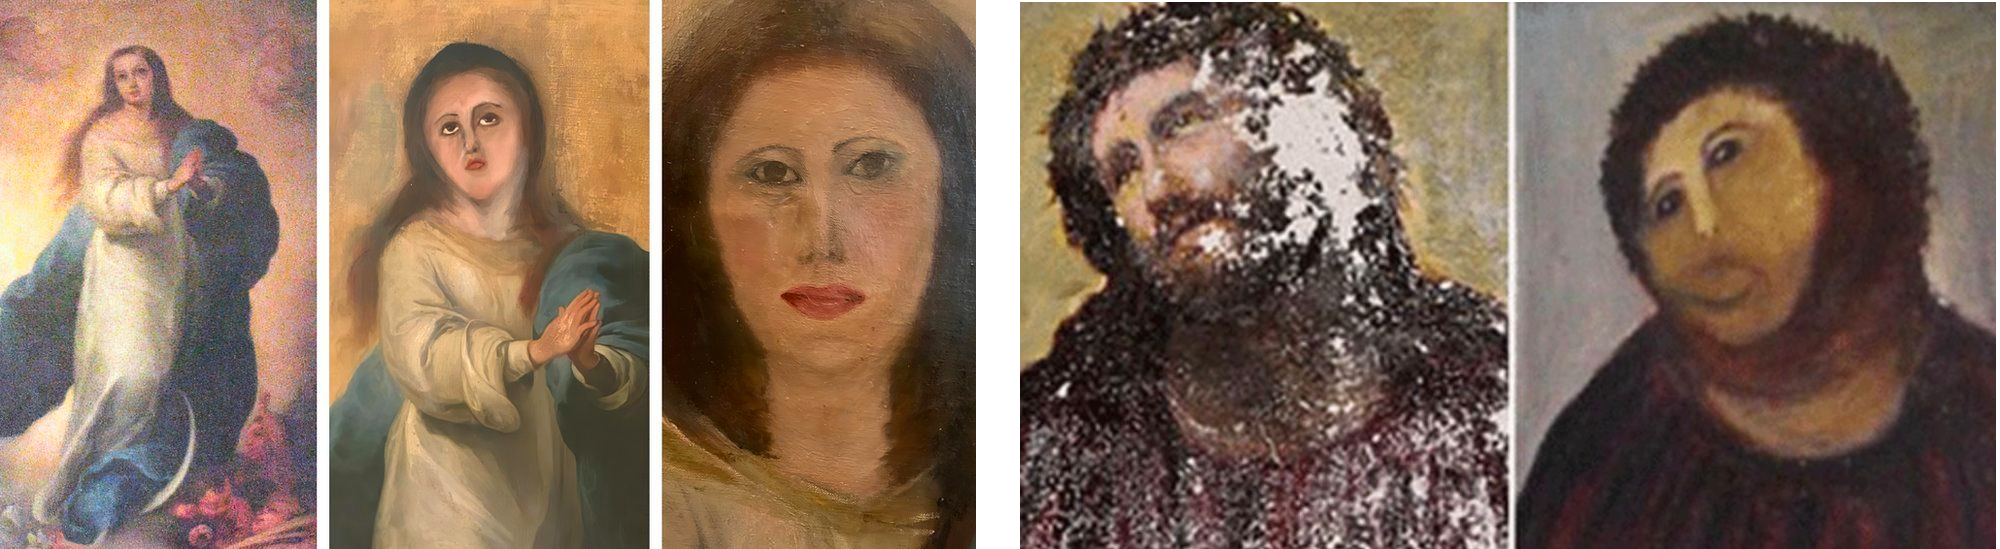
\includegraphics[width=0.87\textwidth]{botched.png}
    \caption{Botched reproductions of Spanish frescoes hand-painted by amateur artists \cite{jesus}}
\end{figure}


\section{Background}
 
\subsection{What is a Convolutional Neural Network?}

A Convolutional Neural Network (CNN) is a type of deep learning method that uses a combination of convolutional layers and pooling layers to make class predictions about an image. First, the convolutional layers produce feature maps by applying a filter across a layer one pixel at a time. Then, the pooling layers ease the computational burden by "summarizing" and reducing the size of feature maps. Finally, these reduced feature maps are passed into a fully connected layer and a prediction is made about an image. 

Depending on the task at hand, a CNN will have different parameters for the activation function, loss function, and optimizer method \cite{mol}\cite{sizyakin}. However, a more technical description of what these parameter changes do is outside the scope of this paper, so it will not be discussed further. 

\subsection{CNNs in Practice}

CNNs have been used in a variety of image-related fields including computer vision, image classification, and image processing. This is because the internal structure of CNNs breaks down the high dimensionality of images into manageable chunks \cite{sizyakin}. Using deep learning to digitally restore artwork is a new field that only came into popular research in the last five or six years, but due to the success of CNNs in other types of image processing tasks, it makes sense that it would have the same success here. It is therefore easy to see in a broad sense why researchers turned to this architecture for art restoration. And as we will see in the next section, there are specific reasons why CNNs have continued to grow in popularity in this field compared to other methods. 

\begin{figure}[h]
    \centering
    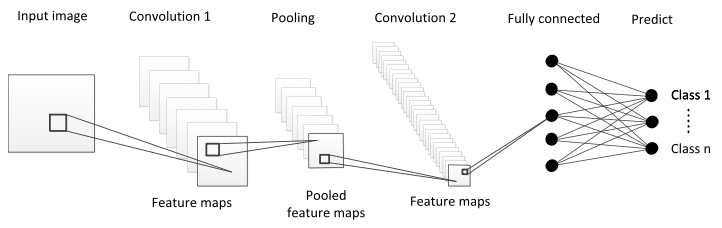
\includegraphics[width=0.87\textwidth]{cnn.png}
    \caption{Structure of a generic CNN classifier. Diagram from Sizyakin et al. \cite{sizyakin}}
\end{figure}
 
\section{Literature Review}

This literature review will have the following structure.  First, we will compare the performance of CNNs vs. early technological reconstructions on three main subtasks: color restoration, crack detection, and image inpainting. The purpose is to examine the ways in which CNNs overcome previous limitations, and thus enhance the quality and efficiency of digital reconstructions. Then, we will examine other advantages of CNNs that are unrelated to the subtasks, but that still contribute to a CNN’s success. These other advantages include accessibility and flexibility. 
 
\subsection{Color Restoration}

One of the most widespread issues that art conservators face is the degradation of color— a problem that arises naturally with age. When old paintings are preserved, they are usually covered with a layer of varnish that protects the artwork from pollutants and dirt \cite{amiri}. However, varnished paintings often yellow as time passes, thus obscuring the natural paint pigments \cite{amiri}\cite{barni2005}. Also, ink drawings, which do not have the protection of varnish, become extremely faded in the light, and the original image can only be inferred from faint, disconnected lines \cite{zeng2018}. By performing digital color restoration on these artworks, we can enhance our own appreciation and visualization of art. 

There have been many methods created to deal with this issue. One early method developed by Barni et al. uses matrix transforms to deal with yellowing \cite{barni2000}. They first clean a small portion of the image by using special cleaning solvents. Then, they find a matrix that can map the cleaned portion of the image to the corresponding uncleaned portion of the image. By applying this transform across the entire image, they can estimate the appearance of the whole painting after cleaning. Pappas et al. similarly modeled the transformation of color, but instead of using matrices, they combined linear approximations and white point \cite{papas}. \footnote{White point” is a set of chromatic values that define the color “white” in an image}

In 2011, Palomero and Soriano became the first researchers to use neural networks for the color restoration task \cite{palomero}. Instead of doing pure color analysis, they were able to identify the varnish as a “filter” over the original painting and estimate the varnish’s spectral reflection. And from this spectral reflection, they could average color data and back-engineer the original colors. But like both the previous approximation methods, Palomero et al. also needed to clean a small section of the painting by hand before applying their color-restoring algorithm. 

As one might guess, the required cleaning step was especially risky for old or delicate paintings that might easily suffer damage from chemicals (Amiri). To combat this, Amiri and Messinger developed an entirely virtual approach using CNNs \cite{amiri}. This approach trains a CNN on artificially yellowed images in order to simulate the color degradation process. In the experiment, Amiri and Messinger took 500 photographs and paintings and covered them with one of three yellow filters ranging from a pale pastel to bright and saturated. Then, they compared the cleaned (non-yellowed) version to the original and tested the Euclidean distance between the two colors. As mentioned, this process was entirely virtual, which makes it more advantageous than the previous methods. Also, instead of just mapping from one color to another, this CNN actually learns the degradation process, making it a smarter solution overall. An example of their method is shown in Figure 3. 

\begin{figure}[h]
    \centering
    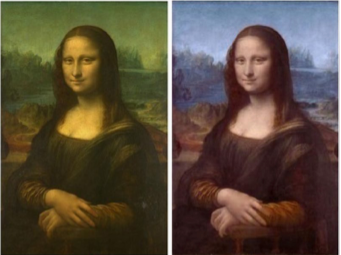
\includegraphics[width=0.5\textwidth]{mona.png}
    \caption{Visualization of \cite{amiri}'s color restoration method. Left is uncleaned Mona Lisa, right is Mona Lisa after cleaning. Image taken from \cite{amiri}}
\end{figure}

Another entirely virtual solution comes from Shankar et al. \cite{shankar}. In this experiment, Shankar et al. prove that CNNs perform well even with severe loss of color, such as with greyscale images. Although these images were virtually greyed, this experiment still shows the capability of CNNs in processing color information, even when there is very little information about the original hue. This is similarly reflected by Zeng et al. \cite{zeng2016}, where they used a CNN to reconstruct color and textural information on severely faded ink drawings. In 2018, they extended these results to show that they could achieve adequate success with the CNN compared to Linear Regression and kNN \cite{zeng2018}.

Finally, since color restoration is often a pixel-wise operation and images can have millions of pixels each \cite{palomero}, methods like kNN can be very inefficient for this task. KNN uses every pixel in the image for its training data, so dealing with high resolution images is extremely cumbersome  \cite{zeng2018}. CNNs, on the other hand, handle high-resolution data well due to their inherent feature reduction, making them an effective solution for color restoration. 


\subsection{Crack Detection/Elimination}

"Cracks" mean places where the artwork is split in a way that disrupts the continuity of the painting. There are no 'missing' portions of the painting as with flaking, but the image is not entirely whole either. There are two common situations in which cracks appear. First, if the painting resides on some cave wall or other organic structure, the rock may crack naturally due to dampness or seismic activity \cite{dulecha}. These cracks can range from hairline fractures to massive fissures. Otherwise, oil-based paints and varnish are prone to cracking as they dry, creating spidery lines that expose the canvas underneath \cite{barni2005}\cite{dulecha}. The detection of cracks is a vital problem in art restoration, as leaving cracks untreated may lead to more severe damage in the painting \cite{dulecha}. In other words, knowing where the cracks are can allow artists to remedy them accordingly by hand. 

Two early solutions for crack detection are filtering-based methods and traditional machine learning methods \cite{agupta}\cite{pizurica}\cite{cornelis}. Filtering-based methods such as the one created by Gupta et al. put grayscale filters over the image and defined cracks as ‘any region exceeding a certain threshold value’ \cite{agupta}. Traditional machine learning methods used vector classification \cite{pizurica}\cite{cornelis}. However, morphological filters details could not easily handle multi-modal data on their own \cite{gupta}. Furthermore, the hand-engineering of features for machine learning approaches made them rather inefficient, even if they were able to handle high-resolution, multimodal data \cite{cornelis}. 

In 2020, Sizyakin et al. developed a CNN-based approach to crack detection that sought to counter some of the major issues with previous methods \cite{sizyakin}. Sizyakin et al. first used morphological filters to eliminate uncracked regions from the Ghent Altarpiece painting. This step reduced the problem size to ensure maximum effectiveness from the CNN, which then took the processed image and defined the individual cracks. In other words, most of the detection steps were done by the CNN, while morphological filters only handled preprocessing. This difference turned out to be quite significant— where the direct application of morphological filters often misidentified bold lines in the painting as damage, the CNN did not have the same issue. Also, the continual reduction of features boosted efficiency in a way that was not possible with traditional machine learning. Finally, while many previous crack detection algorithms widened crack boundaries, Sizyakin's CNN penalized such an action, which not only thinned the identified cracks, but also reduced the amount of undamaged regions that were modified. One result of their method can be seen in Figure 4.

\begin{figure}[h]
    \centering
    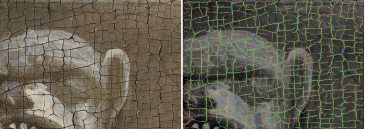
\includegraphics[width=0.65\textwidth]{cracked.png}
    \caption{Visualization of \cite{sizyakin}'s crack detection method. Green is true positives, red is false positives, and blue is false negatives. Image taken from \cite{sizyakin}.}
\end{figure}

Dulecha et al. also used deep learning techniques to detect cracks \cite{dulecha}. Their preprocessing step was done by an edge detection algorithm, while their crack detection was done by a supervised CNN classifier. Similarly to Sizyakin et al., they concluded that the supervised learning approach with CNNs was the best, as it was able to better distinguish between cracks and dark brush strokes in the painting. They also found that their formulation of 6 convolutional layers not only allowed them to outperform traditional neural networks in detecting cracks, but also other CNNs with fewer layers. 


\subsection{Image Inpainting}

Image inpainting involves generating lost portions of an image that either flaked off, tore, or eroded away. Many inpainting methods for artwork use or draw inspiration from inpainting methods for photographs \cite{gupta}. One such method is the PatchMatch algorithm developed by Barnes et al. \cite{barnes}, which for years was considered the state-of-the-art method in image inpainting \cite{gupta}. Using nearest-neighbor approximation, PatchMatch iteratively searches an image for best-fit patches, and uses these patches to fill holes in the image. Although originally used for photographs, this method could be used for paintings as well, with relative success \cite{gupta}. Due to its limited scope, however, PatchMatch could not handle complex shapes/irregularities, nor could it imagine new patterns and designs that exist outside of the source image. Deep neural networks combat the latter by incorporating training data from thousands of sources, which greatly reduces the influence of individual image statistics. 

Gathering thousands of images from the same artist is difficult at best, and impossible at worst. Some researchers attempt to get around this by pooling together pieces from the same artistic movement. By doing so, they can amass a 'general feel' for the style, and are able to use the same CNN on any art that follows the same trends. For instance, to reconstruct the Mogao cave paintings, Zeng et al. used 3000 different samples of Buddhist art from the Mogao walls \cite{zenggongzeng}. Although the paintings were known to be drawn by many different artists, Buddhist paintings from this time period all have a consistent style \cite{li}, and thus the assorted training examples did not drastically hinder the success of their algorithm. In fact, the pooling of all these training examples together gave Zeng et al. an inherent edge over PatchMatch, as there was much more variation and creativity in how the algorithm filled holes. 

In their experiment, Zeng et al. create artificial damage by virtually cutting out rectangles from the paintings (Figure 5). They then conduct a pixel-wise reconstruction of the image, and test the accuracy of their algorithm by comparing the filled rectangles with the original. Other researchers such as Iizuka et al. have also used this method of artificial damage to test their algorithms \cite{iizuka}. In this case, the rectangles were slightly less clean-cut than with Zeng et al. \cite{zenggongzeng}, but they were similarly placed near the center of the image instead of on the edges. The CNNs in either experiment produced viable results for the input images.

\begin{figure}[h]
    \centering
    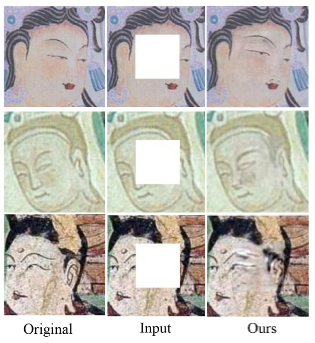
\includegraphics[width=0.48\textwidth]{inp.png}
    \caption{Visualization of \cite{zenggongzeng}'s inpainting method, with rectangles manually removed from the original. Image taken from \cite{zenggongzeng}.}
\end{figure}

As one might guess, however, these perfectly-shaped missing regions (“patches”) are too idealistic. In reality, missing portions of a painting tend to be jagged and/or scattered over multiple regions. Noticing this, Liu et al. used a modified CNN to create a new inpainting technique capable of handling irregular holes in photographs \cite{liu}. By employing the technique from \cite{liu}, Gupta et al. successfully created a CNN to identify these jagged regions \cite{gupta} in paintings as well. This technique could handle polygon-shaped regions or scratches/cracks with ease (Figure 6). These new algorithms not only overcame the main limitations of the PatchMatch method but also the methods created by Zeng et al. \cite{zenggongzeng} and Iizuka et al. \cite{iizuka} by tackling more complex patterns. 


\begin{figure}[h]
    \centering
    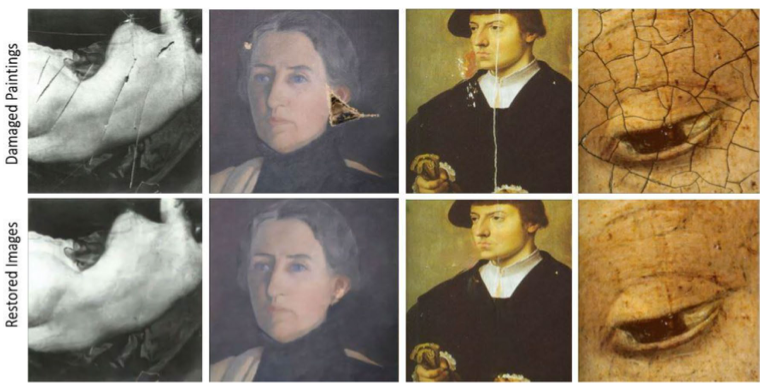
\includegraphics[width=0.67\textwidth]{irreginp.png}
    \caption{Visualization of \cite{gupta}'s inpainting method with paintings suffering from physical damage. Image taken from \cite{gupta}}
\end{figure}



\subsection{Additional Advantages of CNNs}

In addition to their good performance on subtasks, CNNs have other features that contribute to their widespread popularity. This section seeks to outline these other features and explain how and why CNNs outperform early image-processing methods in flexibility and ability to handle complex tasks/patterns at a lower financial cost. 

\subsubsection{Controllable Outputs}

CNNs are compatible with online learning, meaning they can take in additional feedback from experts and have more controllable outputs \cite{zenggongzeng}\cite{sizyakin}. One of the general problems with machine learning/statistical methods is that they are limited in scope. We touched upon this in Section 3.3.3 (“Image Inpainting”) when we mentioned the PatchMatch algorithm from \cite{barnes}. But we include this further analysis to prove that the adaptability of CNNs can improve more than just inpainting techniques. 

Digital art restoration blends together many fields, including optics, color science, computer science, and art history \cite{barni2005}. Online learning acknowledges this by easily incorporating the feedback from scientists and artists all across the world, thus giving the digital restoration a distinctly human touch without needing to move or alter the original painting. For instance, when new annotations become available, Sizyakin’s crack detection approach can efficiently retrain the model to reflect these changes, which makes the program better at generalizing \cite{sizyakin}. Also, the approach by Zeng et al. can provide the model with “examplars” of what the restorer wants the painting to look like \cite{zenggongzeng}. These exemplars produce dynamic outputs that can differ from each other drastically. This way, viewers can experience multiple interpretations of the same artwork, and appreciate the vast diversity of styles that come together to create one art piece. This idea of controllable outputs both improves generalizability and better models human perceptions of aesthetic and restoration techniques.

\subsubsection{Accessibility}

CNNs are more accessible and cost-effective than other digital art restoration methods. In 2008, Elias and Cotte used matrix transforms to produce a highly accurate, virtually cleaned version of DaVinci's Mona Lisa \cite{elias}. This version of the Mona Lisa is considered to be one of the best reproductions out there; because of this, it is even used as a benchmark for the CNN produced by Sizyakin et al. \cite{sizyakin}. This reproduction also proves that methods that do not use machine learning can be very successful. However, the success of their algorithm was largely because they had the financial resources to access the same varnish and pigments that DaVinci himself had used, and were able to leverage that knowledge in their method. All of the other papers outlined in this essay do not share the same privilege, and yet have similar success. This speaks to the vast accessibility of CNNs, and shows how they can achieve more with less financial resources. In fact, this reduced need for expensive tools likely contributes to why CNNs (and deep learning techniques in general) have become so widespread in today’s era. 


\section{Summary \& Conclusion}

\subsection{Results Summary}

The rise of digital solutions has revolutionized art restoration efforts. Although many solutions such as statistical analysis and k-Nearest Neighbors have been proposed and researched, one of the best algorithms for this task thus far has been the Convolutional Neural Network. Convolutional Neural Networks (CNNs) have generally demonstrated good performance in art restoration due to their flexible nature and their ability to handle both complex patterns and high-resolution images with efficiency. As CNNs are entirely virtual, restorers no longer need to move or alter the physical paintings, thus reducing the risk of irreparable damage. These algorithms are also cost-effective, and able to successfully handle some of the most important subtasks in restoration— color restoration, crack detection, and image reconstruction. 

These advantages point to CNNs being some of the most effective virtual restoration techniques to date. Because of CNNs, the quality and availability of digitized restorations have skyrocketed along with the privilege to appreciate art as it was intended to look. Famous paintings such as DaVinci's Mona Lisa, the Ghent Altarpiece, and the Mogao Cave paintings, which are too precious to alter in their original forms, have all benefited from these technologies. Some digital restorations even feature in museums, such as the reconstruction of Rembrandt's 'Night Watch' in Amsterdam's Rijksmuseum \cite{rembrandt}. The original canvas, which had been severed by a knife, now hangs flush with a life-sized print created by a CNN, and the two complement each other to create a full picture. As such, our knowledge and appreciation of this art can continue to flourish and grow. 

\subsection{Future Research}

That’s not to say, however, that the field has stagnated. While CNN-based approaches have dominated thus far, advancements are being made every day in the field of digital restoration, bringing rise to more powerful algorithms. One such promising advancement is the Generative Adversarial Network (GAN). Although GANs may use CNNs inside their algorithm, the two methods are not the same. According to Xiang et al. \cite{xiang} and Cao et al \cite{cao}, GANs perform particularly well on image inpainting tasks— not only can they detect irregular patterns, but they also produce results that align even better to human perceptions of aesthetics than CNNs. GANs are even known for producing hyper-realistic portraits of humans, pointing to a highly successful approach to synthesis \cite{karras} that may aid them massively in art restoration. However, GANs have not been widely studied in digital restoration yet, as they have mostly been applied to photography and real (as opposed to drawn) subjects.

As a final note, something that we must consider for all future research is that humans cannot be removed from the picture. Despite the success of digital restoration, the opinions and skills of artists must be honored— this technology was not meant to replace, but simply to aid. The human factor is why many researchers such as Sizyakin et al. \cite{sizyakin}. and Zeng et al. \cite{zenggongzeng} have begun to expand on online learning techniques for this task. Therefore, methods that are compatible with online learning seem to be the most promising way to combine art conservation and computer science.





%                Now build the reference list
\bibliographystyle{unsrt}   % The reference style
%                This is plain and unsorted, so in the order
%                they appear in the document.


\small
\bibliography{main}       % bib file(s).

\end{document}

